\chapter{The effect of viscosity on the Kelvin-Helmholtz instability in the fan plane of a null point}

\graphicspath{{images/null_point_khi/}}

\section{Introduction}

\subsection{Why are nulls important?}

Null points are an abundant feature in the topologically complex magnetic field of the solar corona [TODO reference to estimate of null points] and are inferred to participate in a number of high-energy phenomena. One such important phenomena is the compact solar flare, thought to arise due to energetic reconnection events occurring in the vicinity of a null, resulting in a flare with a much shorter, brighter life than those associated with coronal loops. Due to the shape of the null, these flares are typically associated with a signatory circular flare ribbon. Null points are also susceptible to collapse, a process that has been theoretically shown to potentially produce oscillatory reconnection TODO ref. The dissipation mechanisms, primarily viscosity and resistivity, can have a strong effect on the dynamic development of the null, particularly the development of reconnection in and around the null point. Aside from the importance of investigating the effect of dissipation on such energetic phenomena, the null point, due to its variation in magnetic field strength, is also an ideal test for the recently developed model of anisotropic viscosity, the switching model. TODO MENTION PRIOR TESTS

Here, we consider an idealised null point which we dynamically stress by twisting the spine. Due to the high speed at which we do this, thin shear layers in the velocity develop along the fan plane which can become unstable to the Kelvin-Helmholtz instability. The vortices created can then go on to promote reconnection in the fan plane. 

\section{Methods}

\subsection{Numerical setup}

The magnetic structure of the null point with the spine aligned along the $z$-axis is written
\begin{equation}
  \label{eq:null_point_field}
  \vec{B} = (x, y, -2z).
\end{equation}
Since we wish to dynamically stress this null point, we let the initial velocity be uniformly zero, $\vec{u} = \vec{0}$. We also set a uniform density $\rho = 1$ and internal energy $\varepsilon = TODO$, corresponding to a temperature of $T = TODO$. At the upper and lower $z$-boundaries we impose a twisting motion centred around the axis of the null with a smooth, $\tanh$-shaped radial profile which is accelerated from stationary using a $\tanh^2$-shaped ramping function. The velocity at the upper boundary is explicitly written as
\begin{equation}
  \label{eq:null_twisting_profile}
  \vec{u} = u_0 u_r(r) u_t(t) (-y, x),
\end{equation}
where $u_r$ describes the radial profile of the twisting motion in terms of the radius $r^2 = x^2 + y^2$,
\begin{equation}
  \label{eq:radial_twisting_function}
  u_r(r) = 1 + \tanh(1 - 36r^2),
\end{equation}
and $u_t(t)$ describes the imposed acceleration of the twisting motion,
\begin{equation}
  \label{eq:ramping_up_function}
  u_t(t) = \tanh^2(t/t_r).
\end{equation}
The peak velocity after the ramping time is approximately $u_0$, At the lower boundary, the flow is in the opposite direction.

\subsection{Tools of analysis}

There are three quantities useful in understanding the stability of the current-vortex sheet. Associated with the shear in velocity and magnetic field are two Mach numbers: the fast mode Mach number, related to the velocity shear, and the projected Alfv\'en Mach number, related to the magnetic shear,
\begin{equation}
  \label{eq:mach_numbers}
  M_f = \frac{\Delta v}{\sqrt{c_s^2 + c_A^2}} \text{and} \quad M_A = \frac{\Delta v \sqrt{rho}}{\Delta B},
\end{equation}
where $\Delta v$ and $\Delta B$ are the respective differences in the velocity and magnetic field over the shear layer, and $c_s$ and $v_A$ are the local sound and Alfv\'en speeds, respectively. Since the shear layer occurs in the presence of a guide field (that of the initial magnetic null point) which does not affect the linear stability of the KHI, we consider the Alfv\'en Mach number projected on to the layer. The parameter describing the balance of stability between the tearing mode and the KHI in a current-vortex sheet is
\begin{equation}
  \label{eq:khi_stability_param}
  \Gamma = \frac{L_b}{L_v} M_A^{2/3}
\end{equation}
where $L_b$ and $L_v$ are the respective widths of the magnetic and velocity shear layers~\cite{einaudiResistiveInstabilitiesFlowing1986}. Again, due to the presence of the guide field, we consider $\Gamma$ projected on to the shear layer. Plotting the radial dependence of these quantities over the shear layers gives an idea of the probable stability. It should be noted that the true stability of the current-vortex sheet studied here also depends on other factors not taken into account by the stability analysis performed by~\cite{einaudiResistiveInstabilitiesFlowing1986} (factors such as viscosity and the presence of a guide field). Hence, these quantities are only an indicator of the stability, not a guarantee.

\section{Results}

\subsection{Evolution of a typical KHI case}
\label{sec:null_point_khi_single_case}

We discuss initially the evolution of the pair of simulations using a resistivity of $\eta = 10^{-4}$ and viscosity $\nu = 10^{-4}$, comparing the two viscosity models. These simulations capture the main features of the null's response to the driver: the formation of a current-vortex sheet in the fan plane, the appearance of counterflows, the growth of a Kelvin-Helmholtz instability, and an eventual null collapse triggered by a fluting instability. This specific choice of parameters also highlights the differences between the isotropic and the switching viscosity models, mainly the suppression of the KHI in the isotropic case.

The total kinetic energy reveals the main developments in the simulations (Figure~\ref{fig:v-4r-4_kinetic_energy}). The initial acceleration of the drivers and injection of torsional Alfv\'en waves occurs between $t=0$ and $2$. After this time the effect of the viscosity models becomes apparent; the energy associated with the KHI grows only in the switching case, peaking between $t=9$ and $10$. Considering only the switching case, the instability generates vortices in the fan plane, encouraging current formation and enhanced Ohmic heating which in turn results in a drop of kinetic energy between $t=10$ and $12$ as the kinetic energy is converted to heat. The current sheets created during the instability also permit small, localised reconnection events, indicated by small peaks in the kinetic energy between $t=10$ and $12$. Over the same time period, the isotropic case remains stable. After $t=12$ a secondary instability, the fluting instability, occurs in both cases. Without the triggering influence of the KHI the isotropic case becomes unstable to the fluting instability at a later time. In turn, the fluting instability triggers the collapse of the null, indicated by the associated spike in kinetic energy at TODO.

\begin{figure}[t]
  \centering
  \includegraphics[width=0.95\linewidth]{v-4r-4_kinetic_energy}
  \caption{}%
  \label{fig:v-4r-4_kinetic_energy}
\end{figure}

Initially, at $t=1$ the torsional Alfv\'en waves injected by the driver trace the field surrounding the null, moving towards the fan plane and out from the spine. The waves eventually meet and create an shear layer in the velocity and magnetic field in the form of a ring of vorticity and current density. Without any diffusion in the system the main wavefronts would travel far along the field before meeting. The presence of both viscosity and resistivity encourages the waves to diffuse as they travel along the field, allowing the upper and lower waves to meet relatively close to the spine, creating rings of shear which are both thicker and smaller in radius. In the switching case, due to the switching model diffusing the field less effectively than the isotropic model, the rings are typically larger in radius, stronger in magnitude, and thinner (Figure~\ref{fig:v-4r-4_vorticity_current_ring_t_3}). Since the viscosity diffuses velocity directly, and affects the magnetic field field through that, the vorticity is affected more than the current density.

\begin{figure}[t]
  \centering
  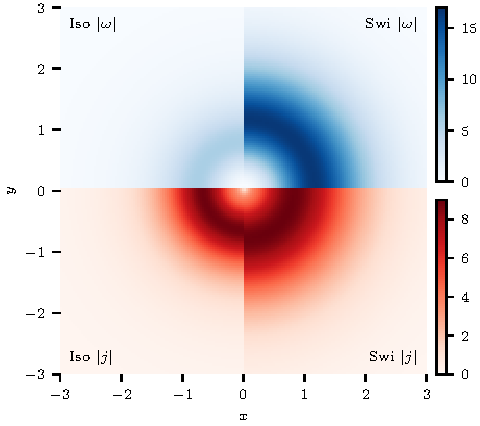
\includegraphics[width=0.48\linewidth]{v-4r-4_vorticity_current_ring_t_3}
  \caption{}%
  \label{fig:v-4r-4_vorticity_current_ring_t_3}
\end{figure}

In the switching case, the velocity shear layer becomes unstable to the KHI, initially presenting as a low-amplitude perturbation overlaying the velocity structure associated with the boundaries (Figure~\ref{fig:v-4r-4_vz_z_0_t_2}). The shear layers created in the isotropic case do not exceed the required stability criteria[TODO expand on this or link back] and remain stable (Figure~\ref{fig:v-4r-4_mach_t_2}). Between times $t=2$ and $6$ magnetic tension opposes the direction of the driver and causes counterflows to appear (Figure~\ref{fig:v-4r-4_counterflows_t_6}) and the current-vortex sheet grows in both size and magnitude, more in the switching case than in the isotropic. The KHI also grows, still only in the switching case. At $t=6$, the reconnection rate is notably higher in the switching case, an indicator of more efficient slippage reconnection due to the lower effective viscosity allowing thinner and stronger current structures TODO FIG line plot of reconnection rate over time.

\begin{figure}[t]
  \centering
  \includegraphics[width=0.8\linewidth]{v-4r-4_vz_z_0_t_2.pdf}
  \caption{}%
  \label{fig:v-4r-4_vz_z_0_t_2}
\end{figure}

\begin{figure}[t]
  \centering
  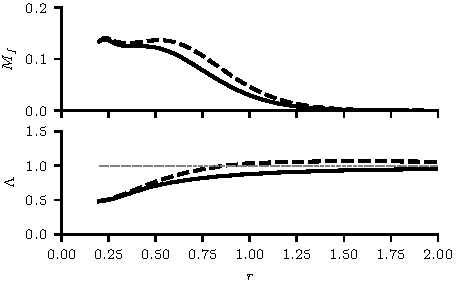
\includegraphics[width=0.9\linewidth]{v-4r-4_mach_t_2.pdf}
  \caption{}%
  \label{fig:v-4r-4_mach_t_2}
\end{figure}

\begin{figure}[t]
  \centering
  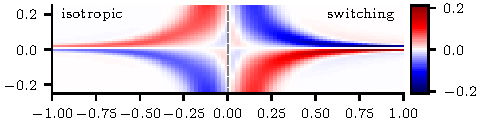
\includegraphics[width=0.9\linewidth]{v-4r-4_counterflows_t_6.pdf}
  \caption{}%
  \label{fig:v-4r-4_counterflows_t_6}
\end{figure}

At $t=7$ the KHI has visibly spread along the fan plane (Figure~\ref{fig:v-4r-4_vz_z_0_t_7}) and by $t=9$ it's clearly visible in the vorticity and current density (Figure~\ref{fig:v-4r-4_vorticity_current_ring_t_9}), although the diagonals are more pronounced due to the effect of the boundaries. The shearing action of the counterflows produces a secondary ring of strong current density closer to the spine. The strength of the current density within the main current-vortex sheet suggests the instability is enhancing the reconnection rate. Indeed, at $t=10$ a branching pattern in the field-integrated parallel electric field provides further evidence for reconnection occurring locally in the rolls of the KHI (Figure~\ref{fig:v-4r-4_reconn_rate_swi_t_10}).

\begin{figure}[t]
  \centering
  \includegraphics[width=0.8\linewidth]{v-4r-4_vz_z_0_t_7.pdf}
  \caption{}%
  \label{fig:v-4r-4_vz_z_0_t_7}
\end{figure}

\begin{figure}[t]
  \centering
  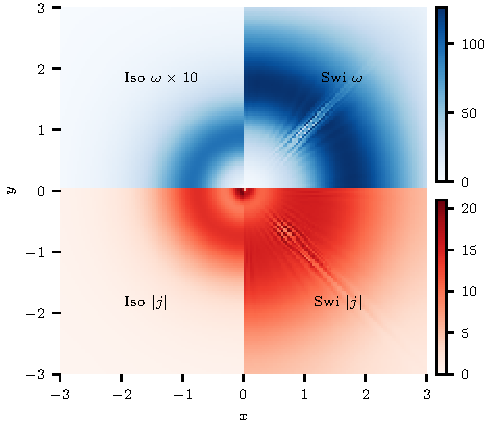
\includegraphics[width=0.48\linewidth]{v-4r-4_vorticity_current_ring_t_9}
  \caption{Note we have multiplied the isotropic vorticity (upper left) by ten to allow comparison.}%
  \label{fig:v-4r-4_vorticity_current_ring_t_9}
\end{figure}

\begin{figure}[t]
  \centering
  \includegraphics[width=0.9\linewidth]{v-4r-4_reconn_rate_swi_t_10.pdf}
  \caption{}%
  \label{fig:v-4r-4_reconn_rate_swi_t_10}
\end{figure}

While the Kelvin-Helmholtz instability grows in the fan plane in the switching case, both cases show growth of another instability located along the spine: the fluting instability. The competition between the inwardly directed magnetic tension in the spine, and the outwardly directed plasma pressure gradient gives rise to an interchange instability. During early stages of the instability, at around $t=6$, magnetic tension increases at four points around the centre axis. The position and number of these points are likely due to the influence of the boundaries. This perturbation in the tension is mirrored by a corresponding perturbation in the thermal pressure which acts to squeeze plasma radially outwards TODO fig of pressure, velocity and magnetic tension (or total force?). The instability continues to grow through $t=10$ with the outflows mixing with the TODO discuss dynamics of instablity after onset. 

Between $t=TODO$ and $t=TODO$ the fluting instability begins to grow (TODO this is different for switching and isotropic how?). Although this instability is influenced by the KHI and seems to influence the eventual collapse of the null, it is not a necessary component of either and so we present the relevant results here and relegate further details to chapter TODO. The instability is generated by the competition between thermal pressure and magnetic tension. 
TODO get story straight about what happens post-flute

At $t=13$ the instability appears to act as a trigger for extremely energetic reconnection in the spine, causing the numerical scheme to display artifacts in locations where the derivatives become too large. The inner

At $t=13$ the null shows some indication of beginning to reconnect and collapse, shown by the presence of velocity structures around the spine, mainly in the isotropic case. The inner ring of current density has shrunk and is now extremely strong, stronger in the isotropic case than the switching case, although we note the current structure located along the spine is around twice as strong as that around the null.

%\begin{figure}[H]
  %\centering
  %\includegraphics[width=0.48\linewidth]{./images/null_point_khi/slices/v-4r-4-isotropic_Velocity_Vx_x_0.0_0013.pdf}
  %\includegraphics[width=0.48\linewidth]{./images/null_point_khi/slices/v-4r-4-switching_Velocity_Vx_x_0.0_0013.pdf}
%\end{figure}

%\begin{figure}[H]
  %\centering
  %\includegraphics[width=0.48\linewidth]{./images/null_point_khi/slices/v-4r-4-isotropic_magnitude_current_density_z_0.0_0013.pdf}
  %\includegraphics[width=0.48\linewidth]{./images/null_point_khi/slices/v-4r-4-switching_magnitude_current_density_z_0.0_0013.pdf}
%\end{figure}

%At $t=14$ in only the isotropic case the ring of density has shrunk entirely to the null.

%\begin{figure}[H]
  %\centering
  %\includegraphics[width=0.48\linewidth]{./images/null_point_khi/slices/v-4r-4-isotropic_magnitude_current_density_z_0.0_0014.pdf}
  %\includegraphics[width=0.48\linewidth]{./images/null_point_khi/slices/v-4r-4-switching_magnitude_current_density_z_0.0_0014.pdf}
%\end{figure}

%At this time, the reconnection rate becomes highly negative at the centre of the plot, in both cases:

%\begin{figure}[H]
  %\centering
  %\includegraphics[width=0.48\linewidth]{./images/null_point_khi/field_line_integrator/v-4r-4-isotropic_integrated_pef_0014.pdf}
  %\includegraphics[width=0.48\linewidth]{./images/null_point_khi/field_line_integrator/v-4r-4-switching_integrated_pef_0014.pdf}
%\end{figure}

%Indeed, by $t=15$, the null is showing signs of collapse in the vorticity, the velocity and in a sudden decrease in current density at the null in the isotropic case.  Note the KHI is still present and the sheer size of the vorticity in the switching case (probably due to a numerical issues, we don't have much stabalising viscous damping in this simulation). It appears as though the presence of the KHI slows the shrinking of the inner current density ring, slowing the eventual collapse of the null.

%\begin{figure}[H]
  %\centering
  %\includegraphics[width=0.48\linewidth]{./images/null_point_khi/slices/v-4r-4-isotropic_vorticity_density_z_0.0_0015.pdf}
  %\includegraphics[width=0.48\linewidth]{./images/null_point_khi/slices/v-4r-4-switching_vorticity_density_z_0.0_0015.pdf}
%\end{figure}

%\begin{figure}[H]
  %\centering
  %\includegraphics[width=0.48\linewidth]{./images/null_point_khi/slices/v-4r-4-isotropic_Velocity_Vz_z_0.0_0015.pdf}
  %\includegraphics[width=0.48\linewidth]{./images/null_point_khi/slices/v-4r-4-switching_Velocity_Vz_z_0.0_0015.pdf}
%\end{figure}

%\begin{figure}[H]
  %\centering
  %\includegraphics[width=0.48\linewidth]{./images/null_point_khi/slices/v-4r-4-isotropic_magnitude_current_density_z_0.0_0015.pdf}
  %\includegraphics[width=0.48\linewidth]{./images/null_point_khi/slices/v-4r-4-switching_magnitude_current_density_z_0.0_0015.pdf}
%\end{figure}

\subsection{Analysis of parameter study}

The results shown in section~\ref{sec:null_point_khi_single_case} do not dramatically change when varying the viscosity $\nu$. However, variation of the resistivity $\eta$ has a strong impact on the dynamics of the stressed null. Generally, increasing $\eta$ to $10^{-3}$ produces a null that remains unstable to the KHI when using switching viscosity, but shows no sign of collapse. In contrast, decreasing $\eta$ to $10^{-5}$ causes the null to collapse much sooner than in the example case in section~\ref{sec:null_point_khi_single_case}. 

eta $10^{-3}$ case - in that the flux of energy injected into the null by the drivers appears to be balanced by dissipative losses [TODO, calculate inputs and outputs]. The effect of the KHI is to increase Ohmic heating through increased reconnection in the fan plane [TODO show this].

One major result to note is that decreasing $\eta$ disrupts the KHI. Although the initial instability can be see in the v-3r-5-switching case (below, left), it does not appear to grow in amplitude and is disrupted by the null collapse which happens much earlier in the low $\eta$ cases, starting between $t=8$ and $9$. Increasing $\eta$ appears to reduce the effect of the boundary, producing a much more radially symmetric KHI (below, right).

TODO check above paragraph in high resolution case. We know the null doesn't collapse as quickly at high res; perhaps the KHI has time to grow.

Throughout many of the simulations $\nu$ does not strongly affect the behaviour in the switching case. The is due to the anisotropic part of the tensor being relatively weak and the isotropic part only being switched on only at the null where there isn't appreciable velocity shears.

In all $\nu = 10^{-3}$ isotropic simulations there's an unexpected, transient artifact in every examined variable. This was also seen in the kink simulations. This is assumed to be due to small-amplitude fast waves created during the initial ramp up, the interaction of which causes the isotropic viscous stress tensor to produce odd effects. It appears to only affect the first time step and slightly increases the viscous heating. Since these results don't differ wildly from those of the $\nu=10{-4}$ simulations we cautiously trust these results.

The stability of KHI in the fan plane is determined via inspection of the out of plane velocity for each parameter choice, resulting in the overview of stability in table~\ref{tab:stability}. The stability and nonlinear development is also reflected in the kinetic energies [TODO 3x3 plot of kinetic energies over all parameter choices]. For resistivities of $10^{-3}$ and $10^{-4}$ using the switching model, there appears a signature growth and decay shape, indicative of the KHI. This is also seen in the single unstable isotropic case, $(\eta, \nu) = (10^{-3}, 10^{-5})$. Isotropic cases $(10^{-3}, 10^{-4})$ and $(10^{-4}, 10^{-3})$ show similar initial increases in kinetic energy, however this does not appear to culminate in instability and we do not notice the small amplitude velocity perturbation seen in other marginally stable cases. Prior to $t = 8$ the kinetic energy in these cases appears similar to the fully unstable cases, but with a more shallow gradient. This is due to TODO WHAT.

\begin{table}[]
\centering
\begin{tabular}{llllll}
$\eta$    & $\nu$    & Magnetic Prandtl number $Pr = \nu/\eta$ & Isotropic Stable? & Switching Stable? &  \\
\midrule
$10^{-5}$ & $10^{-5}$ & $1$ & Stable                 & Unstable*          &  \\
$10^{-5}$ & $10^{-4}$ & $10$ & Stable                 & Unstable*          &  \\
$10^{-5}$ & $10^{-3}$ & $100$ & Stable                 & Unstable*          &  \\
$10^{-4}$ & $10^{-5}$ & $0.1$ & Stable                 & Unstable                 &  \\
$10^{-4}$ & $10^{-4}$ & $1$ & Stable                 & Unstable                 &  \\
$10^{-4}$ & $10^{-3}$ & $10$ & Stable                 & Unstable                 &  \\
$10^{-3}$ & $10^{-5}$ & $0.01$ & Unstable                 & Unstable                 &  \\
$10^{-3}$ & $10^{-4}$ & $0.1$ & Stable                 & Unstable                 &  \\
$10^{-3}$ & $10^{-3}$ & $1$ & Stable                 & Unstable                 & 
\end{tabular}
\caption{Stability in the isotopic and switching cases across varying $\eta$ and $\nu$. The only unstable isotropic simulation is the one corresponding to $\eta = 10^{-3}, \nu = 10^{-5}$. The runs labelled Unstable* refer to simulations where the KHI appears as a small perturbation but does not develop nonlinearly before the null point collapses.}
\label{tab:stability}
\end{table}

The properties of the vorticity and current density rings vary substantially with $\eta$ for both viscosity models and with $\nu$ in only the isotropic case. The lack of dependence on $\nu$ in the switching case is expected since the tensor is nearly zero-valued until the KHI sets in. Generally, both rings increase in radius as $\eta$ and $\nu$ decrease as a result of the upper and lower Alfv\'en waves being able to travel further before diffusing into the fan plane to create the shear layers. Due to the shape of the field, this also allows the rings to appear wider in the radial direction [TODO Does this make sense?]. In the direction out of the fan plane, the thickness of both the current density and vorticity shear layers decreases with decreasing $\eta$ and $\nu$. The respective diffusion parameter naturally affects the shear layer most associated with it, that is resistivity and the current density layer, and viscosity and the vorticity layer. The viscosity generally affects the peak shear in each layer similarly, with the peak magnitude increasing with decreasing $\nu$. This can be attributed to the lack of diffusion at lower $\nu$ allowing the same absolute difference over the shear layer in either velocity or magnetic field to exist in a thinner sheet, resulting in a greater derivative across the layer. In contrast, a decrease in $\eta$ results in a higher peak current density, as expected due to a similar argument as above, but a lower peak vorticity [TODO check this]. This can be attributed to... TODO Generally, the properties of the switching layers could be considered an extreme case of the isotropic results with $\nu$ taken to zero.

TODO plots of thickness, strength and radial extent of current density and vorticity rings

TODO based on ring properties (i.e. mach numbers) why do some runs go unstable and others not?

We now consider the differences apparent in only the switching cases, to investigate the effect of $\nu$ and $\eta$ on the KHI. Before the onset of the KHI the variation in the shear layer properties with $\nu$ are present [TODO are they?] though negligible. Generally, the main differences between simulations with different strengths of viscosity appear during the nonlinear development of the KHI (around $t=9$). After this time, the peaks of both current density and vorticity decrease with decreasing $\nu$ [TODO is this right and if it is why?]. TODO how to show peaks of current density and vorticity? Another plot of peaks after $t=9$? As seen in the example case of section~\ref{sec:null_point_khi_single_case} we find evidence of the KHI promoting slippage reconnection for $\eta = 10^{-3}$ and $10^{-4}$, the two values of $\eta$ that allow the KHI TODO plot of rolls in parallel elec field. Where $\eta=10^{-3}$, the reconnection rate varies little with $\nu$, however the rate increases with decreasing $\nu$ where $\eta=10^{-4}$, caused by TODO WHAT. Alongside the sedate, slippage reconnection, we also find evidence of bursty reconnection in the current density for these value of $\eta$ TODO plot, at $t=TODO$ for $\eta=10^{-3}$ and at the later time of $t=11$ for $\eta=10^{-4}$. Since these current structures are close to grid scale, the accuracy of these results should be viewed with caution, but they are an indicator of the potential for the KHI to promote localised, energetic reconnection events. Both slippage and bursty reconnection is evident in the single KHI-unstable isotropic case, where $\nu=10^{-5}$ and $\eta=10^{-3}$.

\begin{figure}[h]
  \centering
  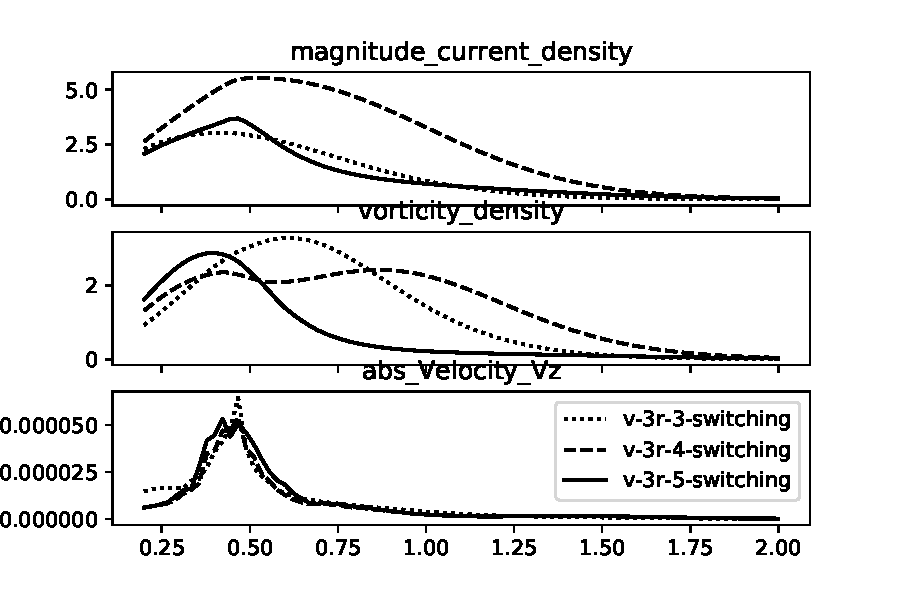
\includegraphics[width=0.8\linewidth]{./images/null_point_khi/azimuthal_averages_v-3_2.pdf}
  \caption{$t=2$}%
  \label{fig:azimuthal_averages_v-3_2}
\end{figure}

\begin{figure}[H]
  \centering
  \includegraphics[width=0.8\linewidth]{./images/null_point_khi/slices/v-3r-5-switching_Velocity_Vz_z_0.0_0002.pdf}
  \caption{$t=2$}%
  \label{fig:v-3r-5-switching_Velocity_Vz_z_0_0002}
\end{figure}

\begin{figure}[h]
  \centering
  \includegraphics[width=0.8\linewidth]{./images/null_point_khi/azimuthal_averages_v-3_4.pdf}
  \caption{$t=4$}%
  \label{fig:azimuthal_averages_v-3_4}
\end{figure}

\begin{figure}[h]
  \centering
  \includegraphics[width=0.8\linewidth]{./images/null_point_khi/azimuthal_averages_v-3_5.pdf}
  \caption{$t=5$}%
  \label{fig:azimuthal_averages_v-3_5}
\end{figure}

\begin{figure}[h]
  \centering
  \includegraphics[width=0.8\linewidth]{./images/null_point_khi/azimuthal_averages_v-3_7.pdf}
  \caption{$t=7$}%
  \label{fig:azimuthal_averages_v-3_7}
\end{figure}

\begin{figure}[h]
  \centering
  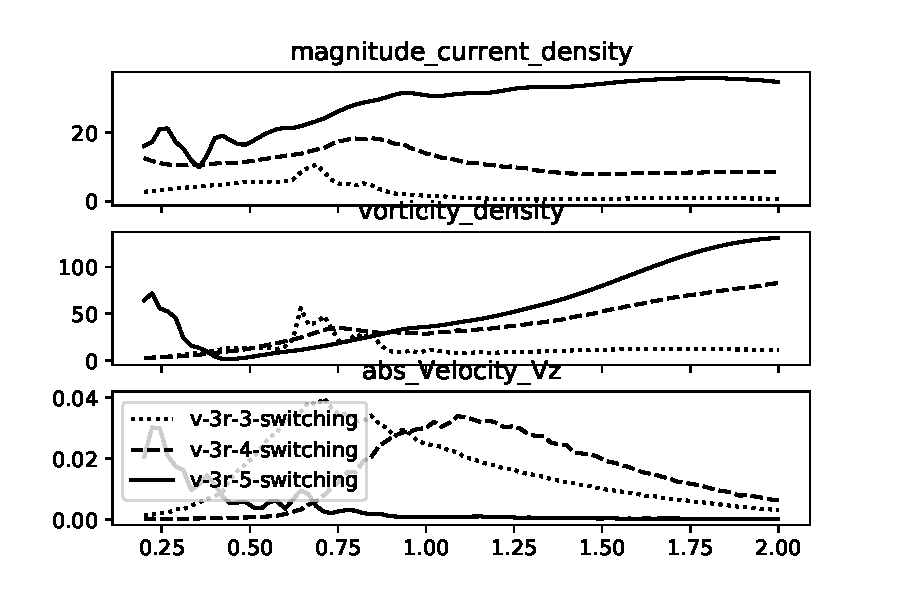
\includegraphics[width=0.8\linewidth]{./images/null_point_khi/azimuthal_averages_v-3_10.pdf}
  \caption{$t=10$}%
  \label{fig:azimuthal_averages_v-3_10}
\end{figure}

Since the value of $\nu$ does not strongly affect the KHI before its nonlinear development, we take the simulation where $\nu = 10^{-3}$ to be representative and focus only on varying $\eta$. We can see the KHI appears as early as $t=2$ in the azimuthally averaged velocity in the $z$-direction, for all three values of $\eta$ (Figure~\ref{fig:azimuthal_averages_v-3_2}) and all at approximately the same location, around $r=0.5$. This can also be clearly seen in the fan plane (Figure TODO properly slice through z of vz at z=0, t=2, v-3r-5), where here $\eta=10{-5}$ but the pattern is similar for other values of $\eta$. Within only two Alfv\'en times it's clear the KHI is able to grow faster when resistivity is greater (Figure~\ref{fig:azimuthal_averages_v-3_4} TODO is this were the figures will end up?). After this time the behaviour for each value of $\eta$ diverges. For high and medium values of $\eta$, the initial instability spreads radially, though more slowly in the medium case. The low, $\eta=10^{-5}$ case shows some evidence of exchange of energy from the magnetic field to the flow, perhaps caused by a small reconnection event, as can be seen from a small dip in the current density colocating with a sudden and transient increase in velocity (Figure~\ref{fig:azimuthal_averages_v-3_4}). This may also be the point at which the isotropic region switches to the switching region (TODO check). If this is the case, the interpolation between the two regions must be made smoother. At $t=7$ the high resistivity case shows further development of the instability (Figure~\ref{fig:azimuthal_averages_v-3_7}). By $t=10$ (Figure~\ref{fig:azimuthal_averages_v-3_10}) the KHI has grown in both high and medium cases, with the energy of the instability peaking at around $r=0.75$ in the high resistivity case, and $r=1.1$ in the medium case.

\begin{figure}[h]
  \centering
  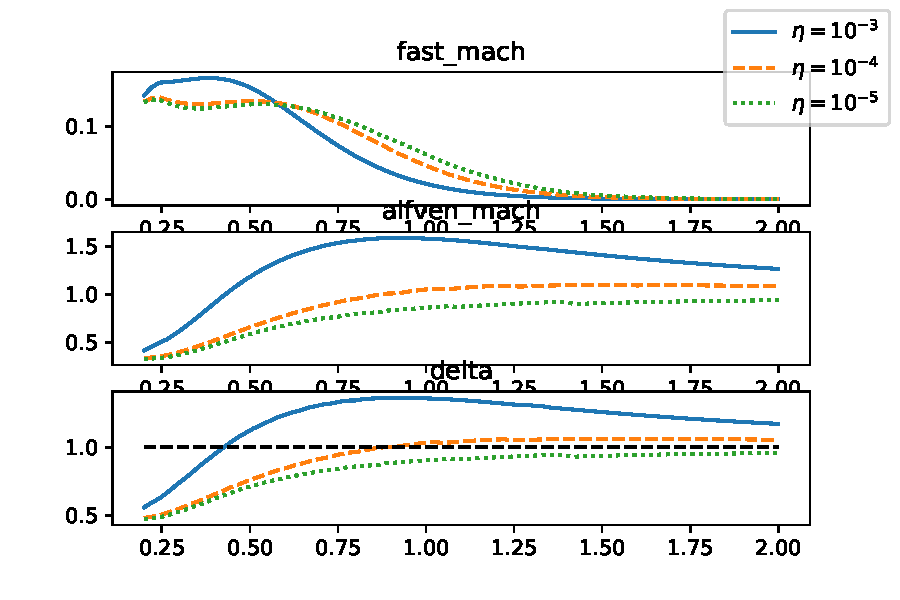
\includegraphics[width=0.8\linewidth]{./images/null_point_khi/mach_numbersv-32.pdf}
  \caption{Mach numbers at $t=2$}
  \label{fig:mach_numbersv_32}
\end{figure}

\begin{figure}[h]
  \centering
  \includegraphics[width=0.8\linewidth]{./images/null_point_khi/mach_numbersv-36.pdf}
  \caption{Mach numbers at $t=6$}
  \label{fig:mach_numbersv-36}
\end{figure}

In order to investigate why the KHI grows so slowly in the low resistivity case, it's instructive to study how the relevant Mach numbers and instability parameters vary radially, and link those to the behaviour and stability of the KHI. As an indicator of the stability of the shear layer, we plot the Mach number associated with the fast-mode $M_f = \frac{\Delta v}{\sqrt{c_s^2 + c_A^2}}$, where $\Delta v$ is the difference in velocity over the shear layer, and $c_s$ and $c_A$ are the local sound and Alfv\'en speeds, respectively, as well as the parameter $\Delta = \frac{L_B}{L_v}(M_{A, proj})^{2/3}$, where $L_B$ and $L_v$ are the widths of the respective magnetic and velocity shear layers, and $M_{A, proj}$ is the Alfv\'en velocity of the layer after removing the guide field, i.e. $M_{A, proj} = \frac{\Delta v \sqrt{\rho}}{\Delta B}$ (TODO reword this entire sentence). For the layer to be unstable to the KHI, $M_f < 2$ and $\Delta > 1$. At early times ($t=2$) the initial growth of the instability occurs at $r=0.5$, coinciding with the peak of $M_f$ (Figure~\ref{fig:mach_numbersv_32}). At this time and location, it is only the high resistivity case which shows shear layers with $\Delta > 1$. Both lower resistivity cases are linearly stable to the instability. This changes for the mid resistivity case (TODO decide mid or medium) only around $t=6$ (Figure~\ref{fig:mach_numbersv-36}), where the peak of $M_f$ coincides with the point where $\Delta \approx 1$ and the instability begins to grow.

TODO what is the behaviour of the fluting instability in all cases?

TODO For which parameters does the null collapse and what does the reconnection look like?

For $\eta=10^{-5}$, the reconnection rate is generally higher than the $10^{-4}$ simulations, particularly along the field lines that intersect the vorticity-current density ring, and along the spine until a reconnection event occurs around $t=10$ in the isotropic cases. The strength of the resultant outflows depend strongly on $\nu$, as does the proceeding reconnection within the rest of the structure, the rate of which is generally higher for weaker viscosity. In the switching case, the initial reconnection event appears sooner and, while the reconnection rate remains relatively constant across the range of $\nu$, lower viscosity does lead to a more violent resultant behaviour.
